\documentclass[paper=letter,11pt]{scrartcl}

\KOMAoptions{headinclude=true, footinclude=false}
\KOMAoptions{DIV=14, BCOR=5mm}
\KOMAoptions{numbers=noendperiod}
\KOMAoptions{parskip=half}
\addtokomafont{disposition}{\rmfamily}
\addtokomafont{part}{\LARGE}
\addtokomafont{descriptionlabel}{\rmfamily}
%\setkomafont{pageheadfoot}{\normalsize\sffamily}
\setkomafont{pagehead}{\normalsize\rmfamily}
%\setkomafont{publishers}{\normalsize\rmfamily}
\setkomafont{caption}{\normalfont\small}
\setcapindent{0pt}
\deffootnote[1em]{1em}{1em}{\textsuperscript{\thefootnotemark}\ }


\usepackage{amsmath}
\usepackage[varg]{txfonts}
\usepackage[T1]{fontenc}
\usepackage{graphicx}
\usepackage{xcolor}
\usepackage[american]{babel}
% hyperref is needed in many places, so include it here
\usepackage{hyperref}

\usepackage{xspace}
\usepackage{multirow}
\usepackage{float}


\usepackage{braket}
\usepackage{bbm}
\usepackage{relsize}
\usepackage{tcolorbox}

\def\ketY{\ensuremath{\ket {\Psi}}}
\def\iGeV{\ensuremath{\textrm{GeV}^{-1}}}
%\def\mp{\ensuremath{m_{\textrm{proton}}}}
\def\rp{\ensuremath{r_{\textrm{proton}}}}
\def\me{\ensuremath{m_{\textrm{electron}}}}
\def\aG{\ensuremath{\alpha_G}}
\def\rAtom{\ensuremath{r_{\textrm{atom}}}}
\def\rNucl{\ensuremath{r_{\textrm{nucleus}}}}
\def\GN{\ensuremath{\textrm{G}_\textrm{N}}}
\def\ketX{\ensuremath{\ket{\vec{x}}}}
\def\ve{\ensuremath{\vec{\epsilon}}}


\def\ABCDMatrix{\ensuremath{\begin{pmatrix} A &  B  \\ C  & D \end{pmatrix}}}
\def\xyprime{\ensuremath{\begin{pmatrix} x' \\ y' \end{pmatrix}}}
\def\xyprimeT{\ensuremath{\begin{pmatrix} x' &  y' \end{pmatrix}}}
\def\xy{\ensuremath{\begin{pmatrix} x \\ y \end{pmatrix}}}
\def\xyT{\ensuremath{\begin{pmatrix} x & y \end{pmatrix}}}

\def\IMatrix{\ensuremath{\begin{pmatrix} 0 &  1  \\ -1  & 0 \end{pmatrix}}}
\def\IBoostMatrix{\ensuremath{\begin{pmatrix} 0 &  1  \\ 1  & 0 \end{pmatrix}}}
\def\JThree{\ensuremath{\begin{pmatrix}    0 & -i & 0  \\ i & 0  & 0 \\ 0 & 0 & 0 \end{pmatrix}}} 
\def\JTwo{\ensuremath{\begin{bmatrix}    0 & 0 & -i  \\ 0 & 0  & 0 \\ i & 0 & 0 \end{bmatrix}}}
\def\JOne{\ensuremath{\begin{bmatrix}    0 & 0 & 0  \\ 0 & 0  & -i \\ 0 & i & 0 \end{bmatrix}}}
\def\etamn{\ensuremath{\eta_{\mu\nu}}}
\def\Lmn{\ensuremath{\Lambda^\mu_\nu}}
\def\dmn{\ensuremath{\delta^\mu_\nu}}
\def\wmn{\ensuremath{\omega^\mu_\nu}}
\def\be{\begin{equation*}}
\def\ee{\end{equation*}}
\def\bea{\begin{eqnarray*}}
\def\eea{\end{eqnarray*}}
\def\bi{\begin{itemize}}
\def\ei{\end{itemize}}
\def\fmn{\ensuremath{F_{\mu\nu}}}
\def\fMN{\ensuremath{F^{\mu\nu}}}
\def\bc{\begin{center}}
\def\ec{\end{center}}
\def\nus{$\nu$s}

\def\adagger{\ensuremath{a_{p\sigma}^\dagger}}
\def\lineacross{\noindent\rule{\textwidth}{1pt}}

\newcommand{\multiline}[1] {
\begin{tabular} {|l}
#1
\end{tabular}
}

\newcommand{\multilineNoLine}[1] {
\begin{tabular} {l}
#1
\end{tabular}
}



\newcommand{\lineTwo}[2] {
\begin{tabular} {|l}
#1 \\
#2
\end{tabular}
}

\newcommand{\rmt}[1] {
\textrm{#1}
}


%
% Units
%
\def\m{\ensuremath{\rmt{m}}}
\def\GeV{\ensuremath{\rmt{GeV}}}
\def\pt{\ensuremath{p_\rmt{T}}}


\def\parity{\ensuremath{\mathcal{P}}}

\usepackage{cancel}
\usepackage{ mathrsfs }
\def\bigL{\ensuremath{\mathscr{L}}}

\usepackage{ dsfont }



\usepackage{fancyhdr}
\fancyhf{}

\usepackage{braket}

\def\ketY{\ensuremath{\ket {\Psi}}}
\def\iGeV{\ensuremath{\textrm{GeV}^{-1}}}
%\def\mp{\ensuremath{m_{\textrm{proton}}}}
\def\rp{\ensuremath{r_{\textrm{proton}}}}
\def\me{\ensuremath{m_{\textrm{electron}}}}
\def\aG{\ensuremath{\alpha_G}}
\def\rAtom{\ensuremath{r_{\textrm{atom}}}}
\def\rNucl{\ensuremath{r_{\textrm{nucleus}}}}
\def\GN{\ensuremath{\textrm{G}_\textrm{N}}}
\def\ketX{\ensuremath{\ket{\vec{x}}}}
\def\ve{\ensuremath{\vec{\epsilon}}}


\def\ABCDMatrix{\ensuremath{\begin{pmatrix} A &  B  \\ C  & D \end{pmatrix}}}
\def\xyprime{\ensuremath{\begin{pmatrix} x' \\ y' \end{pmatrix}}}
\def\xyprimeT{\ensuremath{\begin{pmatrix} x' &  y' \end{pmatrix}}}
\def\xy{\ensuremath{\begin{pmatrix} x \\ y \end{pmatrix}}}
\def\xyT{\ensuremath{\begin{pmatrix} x & y \end{pmatrix}}}

\def\IMatrix{\ensuremath{\begin{pmatrix} 0 &  1  \\ -1  & 0 \end{pmatrix}}}
\def\IBoostMatrix{\ensuremath{\begin{pmatrix} 0 &  1  \\ 1  & 0 \end{pmatrix}}}
\def\JThree{\ensuremath{\begin{pmatrix}    0 & -i & 0  \\ i & 0  & 0 \\ 0 & 0 & 0 \end{pmatrix}}} 
\def\JTwo{\ensuremath{\begin{bmatrix}    0 & 0 & -i  \\ 0 & 0  & 0 \\ i & 0 & 0 \end{bmatrix}}}
\def\JOne{\ensuremath{\begin{bmatrix}    0 & 0 & 0  \\ 0 & 0  & -i \\ 0 & i & 0 \end{bmatrix}}}
\def\etamn{\ensuremath{\eta_{\mu\nu}}}
\def\Lmn{\ensuremath{\Lambda^\mu_\nu}}
\def\dmn{\ensuremath{\delta^\mu_\nu}}
\def\wmn{\ensuremath{\omega^\mu_\nu}}
\def\be{\begin{equation*}}
\def\ee{\end{equation*}}
\def\bea{\begin{eqnarray*}}
\def\eea{\end{eqnarray*}}
\def\bi{\begin{itemize}}
\def\ei{\end{itemize}}
\def\fmn{\ensuremath{F_{\mu\nu}}}
\def\fMN{\ensuremath{F^{\mu\nu}}}
\def\bc{\begin{center}}
\def\ec{\end{center}}
\def\nus{$\nu$s}

\def\adagger{\ensuremath{a_{p\sigma}^\dagger}}
\def\lineacross{\noindent\rule{\textwidth}{1pt}}

\newcommand{\multiline}[1] {
\begin{tabular} {|l}
#1
\end{tabular}
}

\newcommand{\multilineNoLine}[1] {
\begin{tabular} {l}
#1
\end{tabular}
}



\newcommand{\lineTwo}[2] {
\begin{tabular} {|l}
#1 \\
#2
\end{tabular}
}

\newcommand{\rmt}[1] {
\textrm{#1}
}


%
% Units
%
\def\m{\ensuremath{\rmt{m}}}
\def\GeV{\ensuremath{\rmt{GeV}}}
\def\pt{\ensuremath{p_\rmt{T}}}


\def\parity{\ensuremath{\mathcal{P}}}

\usepackage{cancel}
\usepackage{ mathrsfs }
\def\bigL{\ensuremath{\mathscr{L}}}

\usepackage{ dsfont }




\usepackage{fancyhdr}
\usepackage{cancel}
\usepackage{ mathrsfs }





\fancyhf{}
\lhead{\Large 33-444} % \hfill Introduction to Particle Physics \hfill Spring 2020}
\chead{\Large Introduction to Particle Physics} % \hfill Spring 2020}
\rhead{\Large Spring 2020} % \hfill Introduction to Particle Physics \hfill Spring 2020}
\begin{document}
\thispagestyle{fancy}





%\begin{tabular}{c}
%{\large 33-444 \hfill Intro To Particle \hfill Spring 2020\\}
%\hline 
%\end{tabular}

\begin{center}
{\huge \textbf{Homework Set \#8 }}
\large

{\textbf{ Due Date:} Friday March 27th  } 
\end{center}

{\large

\textbf{1) Z boson decays: } \hfill \textit{(5 points)}\\

We assumed that the Z-couplings were universal, that the phase space intergrals were the same for all decay products, and that no higher-order diagrams were relevant. 
(The phase space intergrals will be the same if we can neglect the decay products masses.)

\be
Br(Z\rightarrow ee) \sim \frac{1}{21} = 0.048 \rmt{ vs } 0.034  \rmt{ in PDG }
\ee

\be
Br(Z\rightarrow bb) \sim \frac{3}{21} = 0.143 \rmt{ vs } 0.156  \rmt{ in PDG }
\ee


\textbf{2) Muon decays: } \hfill \textit{(10 points)}\\
\begin{itemize}
\item[a)]{ ${ }$\\
\bc
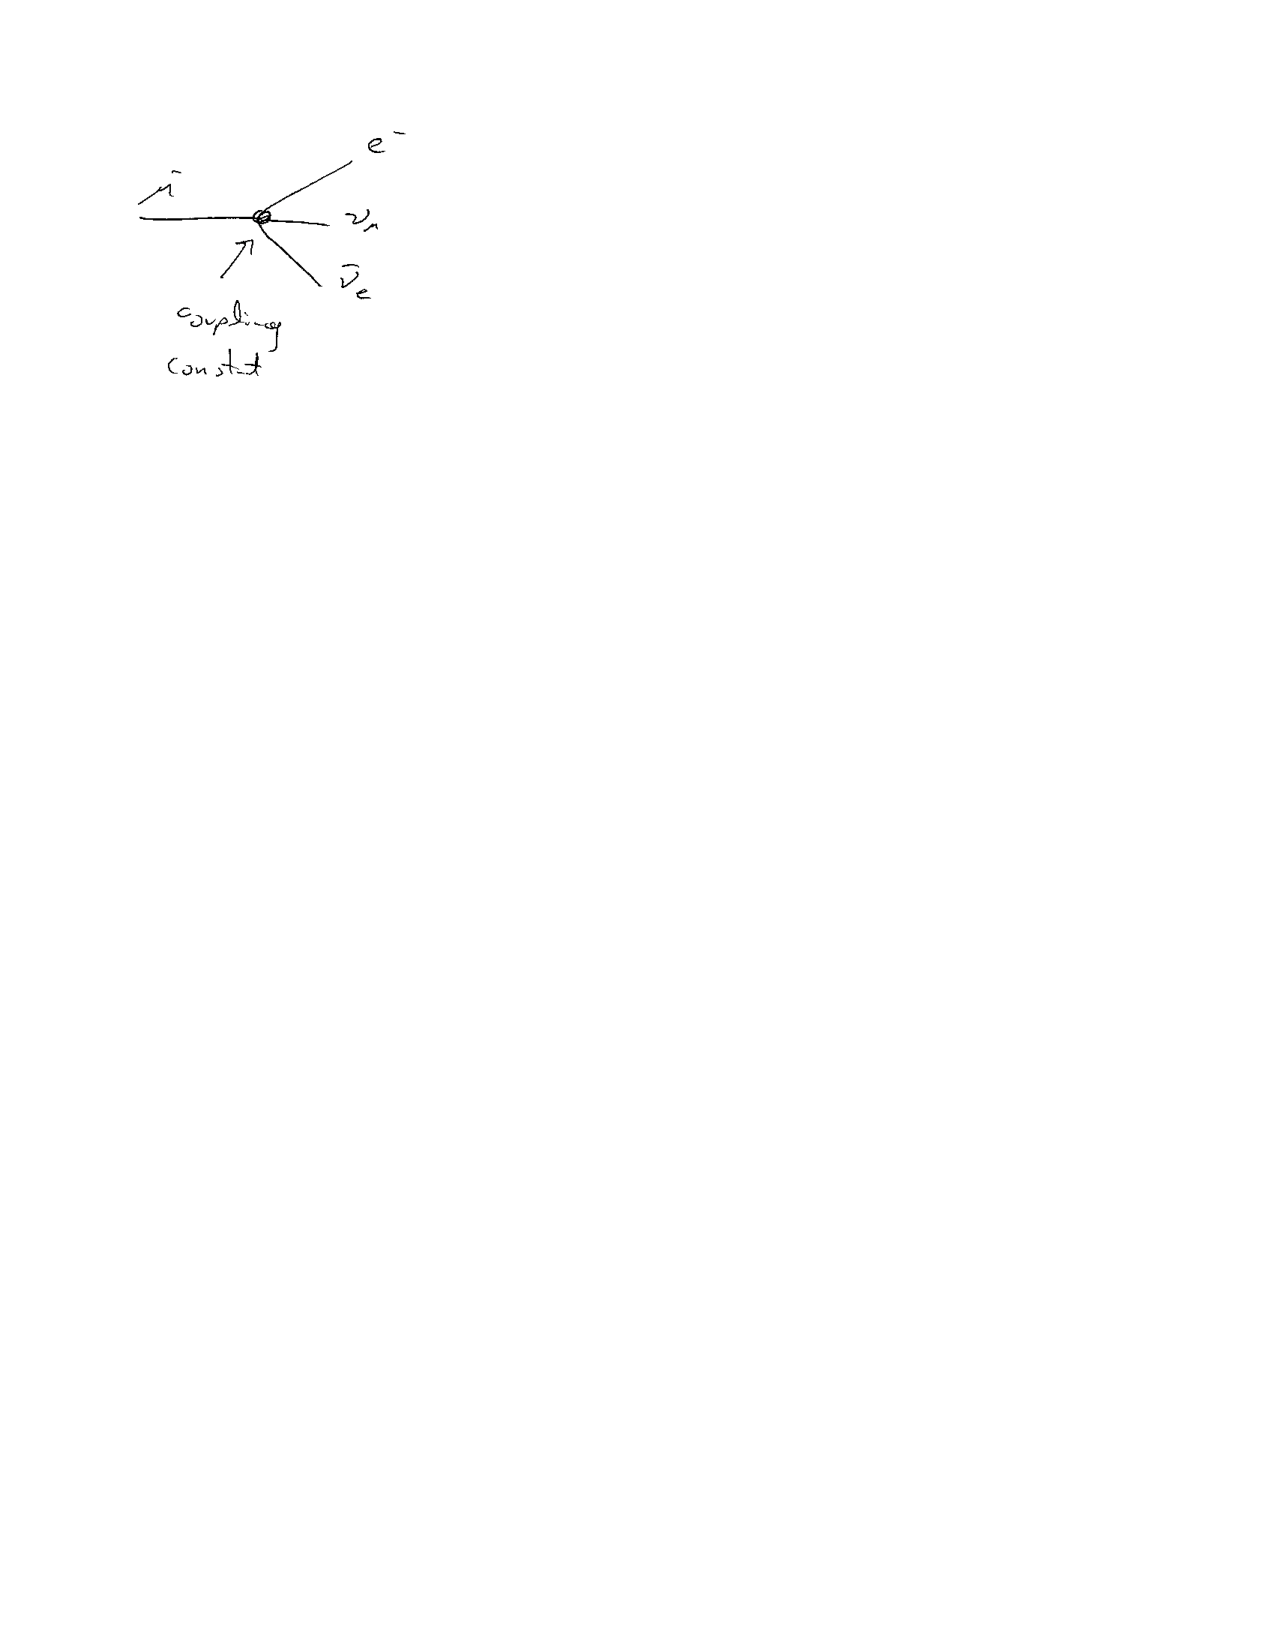
\includegraphics[width=0.3\textwidth]{./4pointInteraction.pdf}
\ec
}

\item[b)]{ We have 4-bosons (each of dim 3/2)  and the coupling constant.  The total dimensions have to add up to 4. 

\be
4 \times \frac{3}{2} + \rmt{[coupling constant]} = 4
\ee

$\Rightarrow$
\be
 \rmt{[coupling constant]} \sim  -2\ \rmt{or}\ \GeV^{-2}
\ee

}

\item[c)]{ 

\be
\Gamma \sim |M|^2 \sim  \rmt{[coupling constant]}^2 = \GeV^{-4}
\ee
}
But we also know that $\Gamma$ has to come out to have overall dimensions of $\frac{1}{\rmt{time}}$ or \GeV.

$\Rightarrow$  
\be
\Gamma \sim m_\mu^5
\ee

\item[d)]{
$m_\mu \sim 0.1 \GeV$, $m_\tau \sim 1 \GeV$, $\tau_\mu \sim 1\mu s$

Now from c) 
\be
\Gamma_\tau \sim m_\tau^5
\ee

and we know
\bea
\tau_\mu = \Gamma_\mu^{-1}\\
\tau_\tau = \Gamma_\tau^{-1}
\eea

so, 

\be
\frac{\tau_\tau}{\tau_\mu} = \frac{\Gamma_\mu}{\Gamma_\tau}
\ee

$\Rightarrow$
\be
\tau_\tau = \tau_\mu \frac{\Gamma_\mu}{\Gamma_\tau} = \tau_\mu \frac{m_\mu^5}{m_\tau^5} = \tau_\mu \left(\frac{m_\mu}{m_\tau}\right)^5  = 1\mu s (10^{-1})^5 = 10^{-6} s \times 10^{-5} = 10^{-11} s
\ee
}

\item[e)]{
with a direct three-point $\mu \rightarrow e \gamma$ vertex, the only mass scale is $m_\mu$. (b/c the ($\mu e \gamma$)- coupling  is dimensionless)

So, $\Gamma_{\mu\rightarrow e \gamma} \sim m_\mu$ (to get the dimensions on $\Gamma$ right)

We know from above that with the four-point interaction in Fermi theory $\Gamma_{SM} \sim m_\mu^5 m_W^{-4}$

So,

\be
\frac{\tau_{new}}{\tau_{SM}} \sim \frac{m_\mu^5 m_W^{-4}}{m_\mu} \sim \left(\frac{m_\mu}{m_W}\right)^4 \sim \left(\frac{0.1\ \GeV}{100\ \GeV}\right)^4  \sim 10^{12}
\ee

The direct $\mu \rightarrow e \gamma$ would dominate (by a factor  $10^{12}$!)\\
The weak interaction is damned weak.

}
\end{itemize}

\clearpage

%
%  New Force
%
\textbf{3) A new force. } \hfill \textit{(5 points)}\\

\begin{itemize}
\item[a)]{ ${ }$\\
\bc
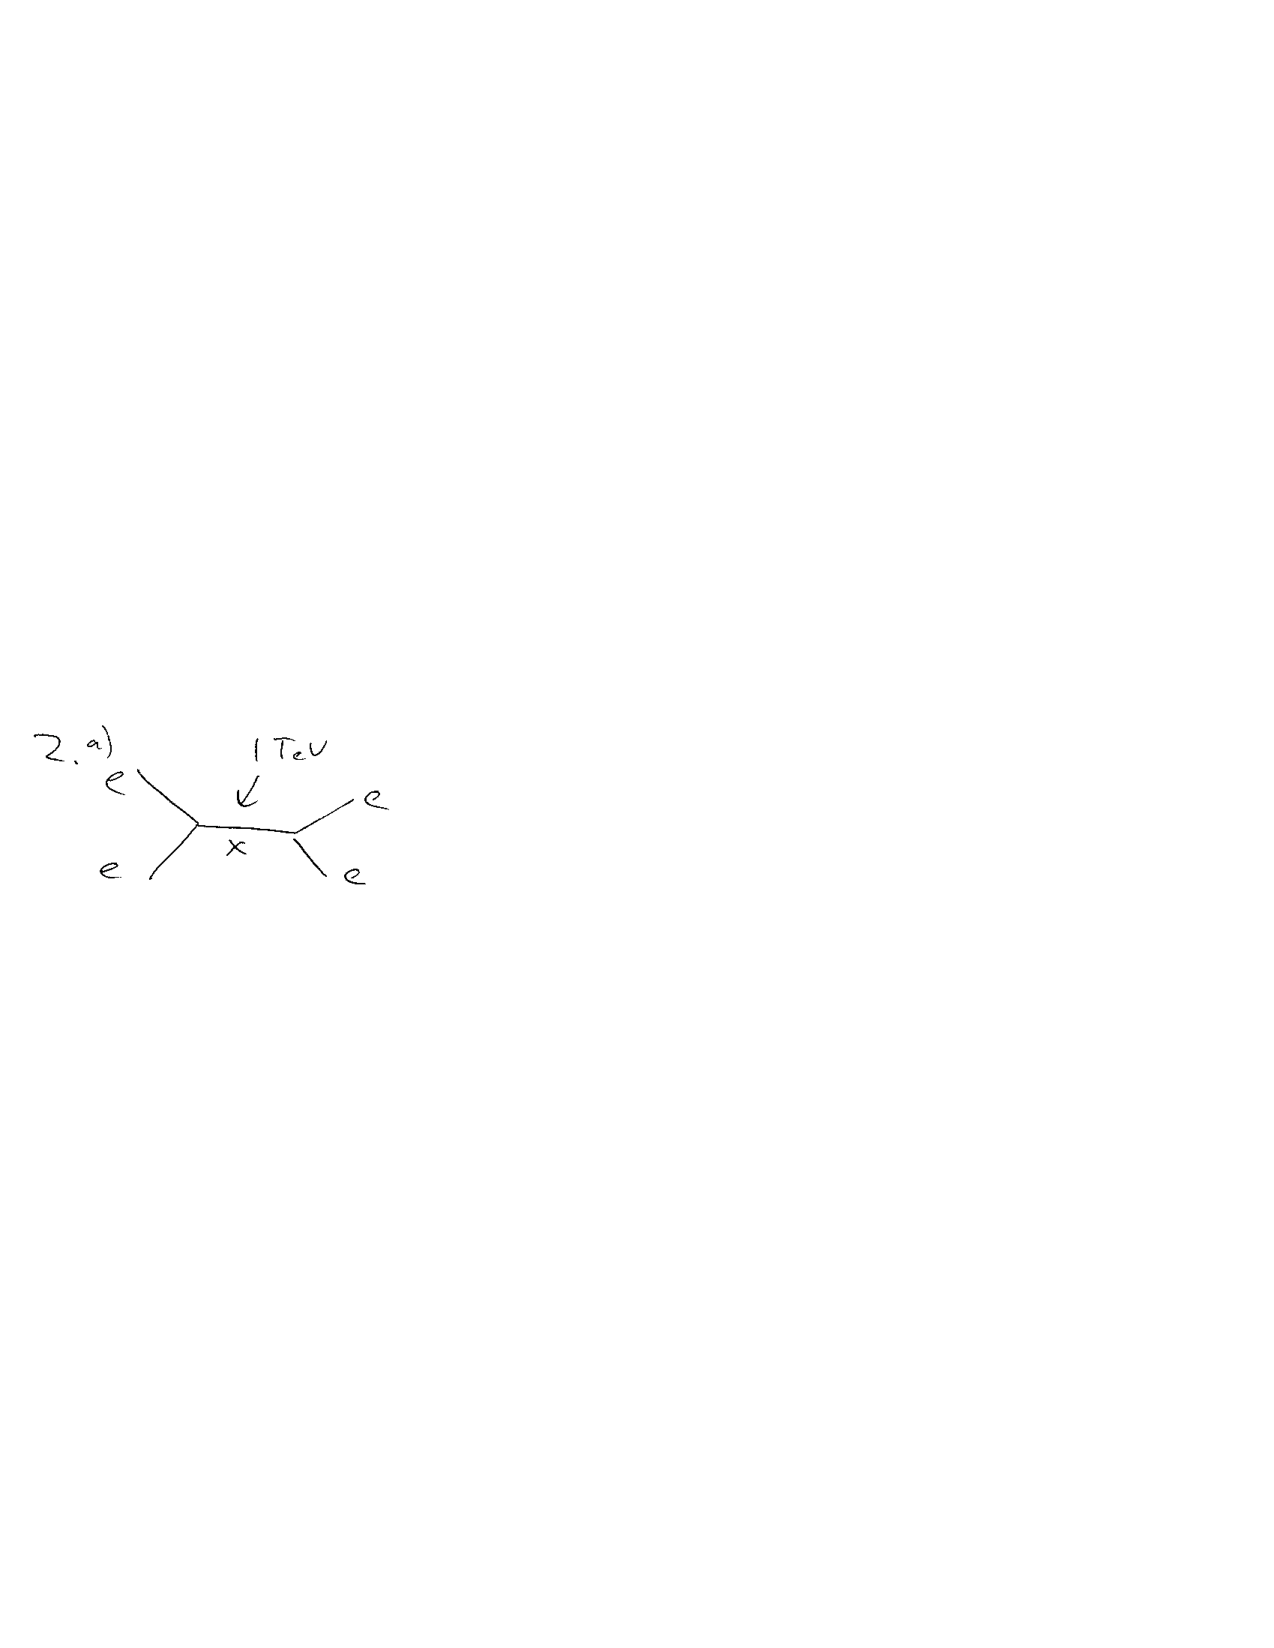
\includegraphics[width=0.3\textwidth]{./eeXee.pdf}
\ec
Range $\sim \frac{1}{m_X} \sim \frac{1}{1000 \GeV} \sim 10^{-3}\ \GeV^{-1} \sim 10^{-19}\ m$
}

\item[b)]{ ${ }$\\
\bc
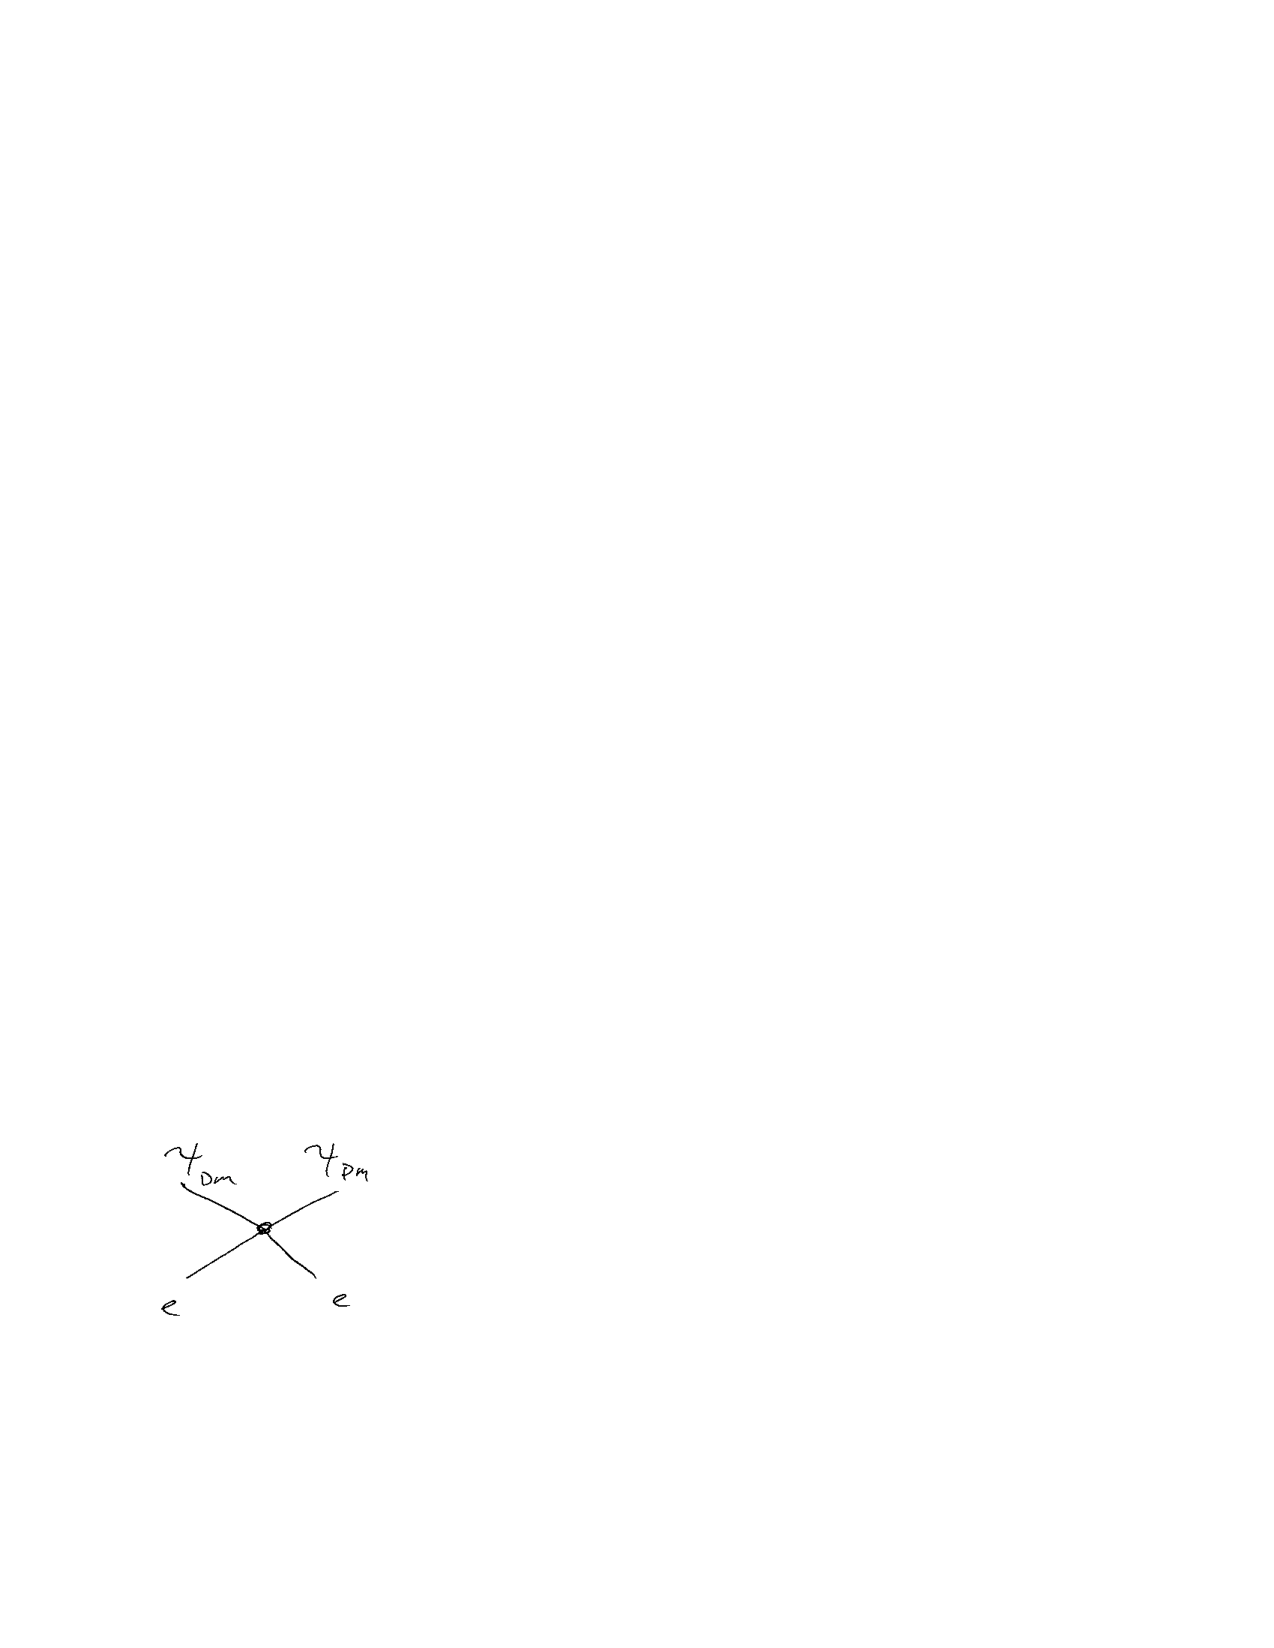
\includegraphics[width=0.2\textwidth]{./eeDmDm.pdf}
\ec

Four fermion interaction $\Rightarrow$ Units of coupliing $\GeV^{-2} \sim \frac{1}{m_X^2}$ 

}


\item[c)]{ ${ }$\\
\bc
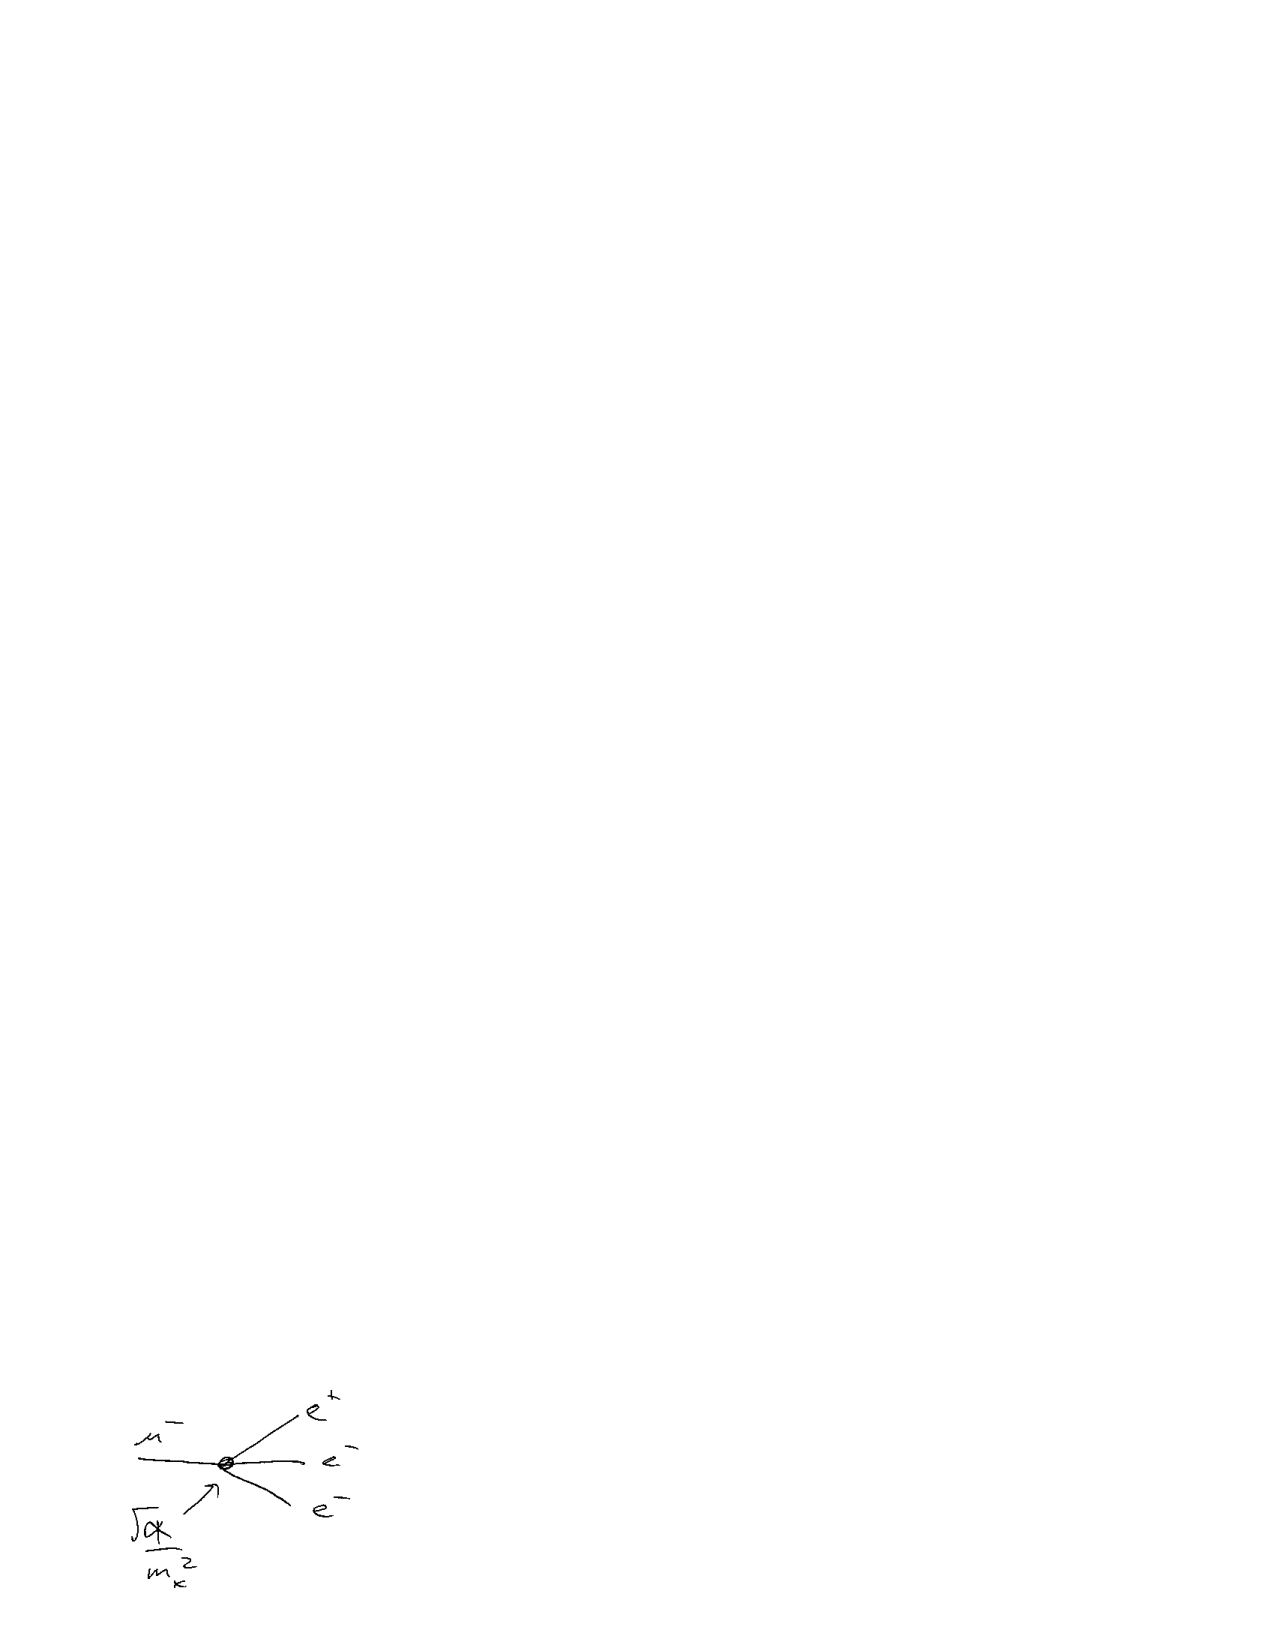
\includegraphics[width=0.3\textwidth]{./muDecayX.pdf}
\ec

\be
\Gamma_{\rmt{New}} \sim \frac{m_\mu^5}{m_X^4} \hspace*{0.5in} \rmt{(see problem 2 for login on why $m_\mu^5$)}
\ee


\be
\Gamma_{\rmt{SM}} \sim \frac{m_\mu^5}{m_W^4}  \hspace*{0.5in} \rmt{(from problem 2)}
\ee

So,
\be
\frac{\tau_{\rmt{New}}}{\tau_{\rmt{SM}}} \sim \left(\frac{m_X}{m_w} \right)^4 \sim 10^4
\ee
$\Rightarrow$ SM decays dominate!
}

\end{itemize}



\textbf{4)  $W$ boson decays to electrons. } \hfill \textit{(3 points)}\\
\begin{itemize}
\item[a)]{ The W can decay directly to an electron or to electron by decaying through a $\tau$. Draw the corresponding diagrams.
\bc
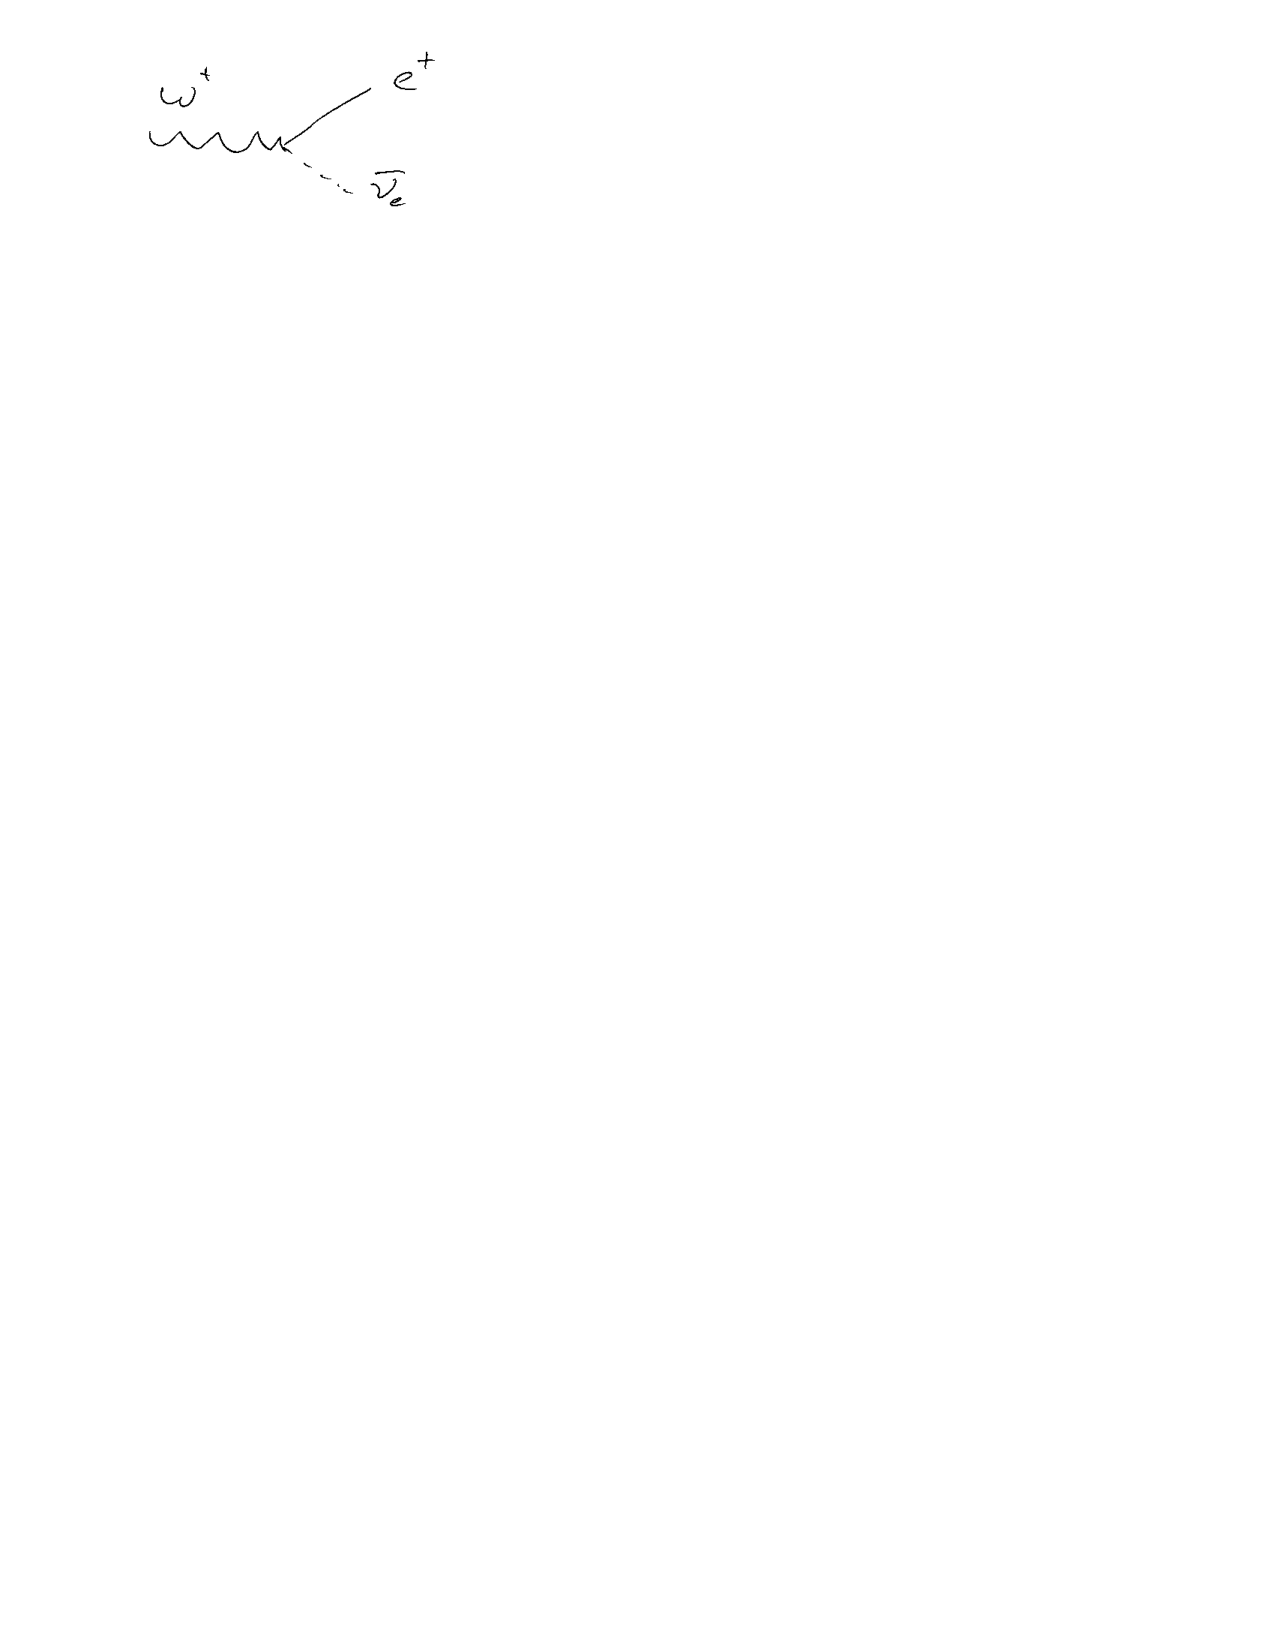
\includegraphics[width=0.3\textwidth]{./Wenu.pdf}
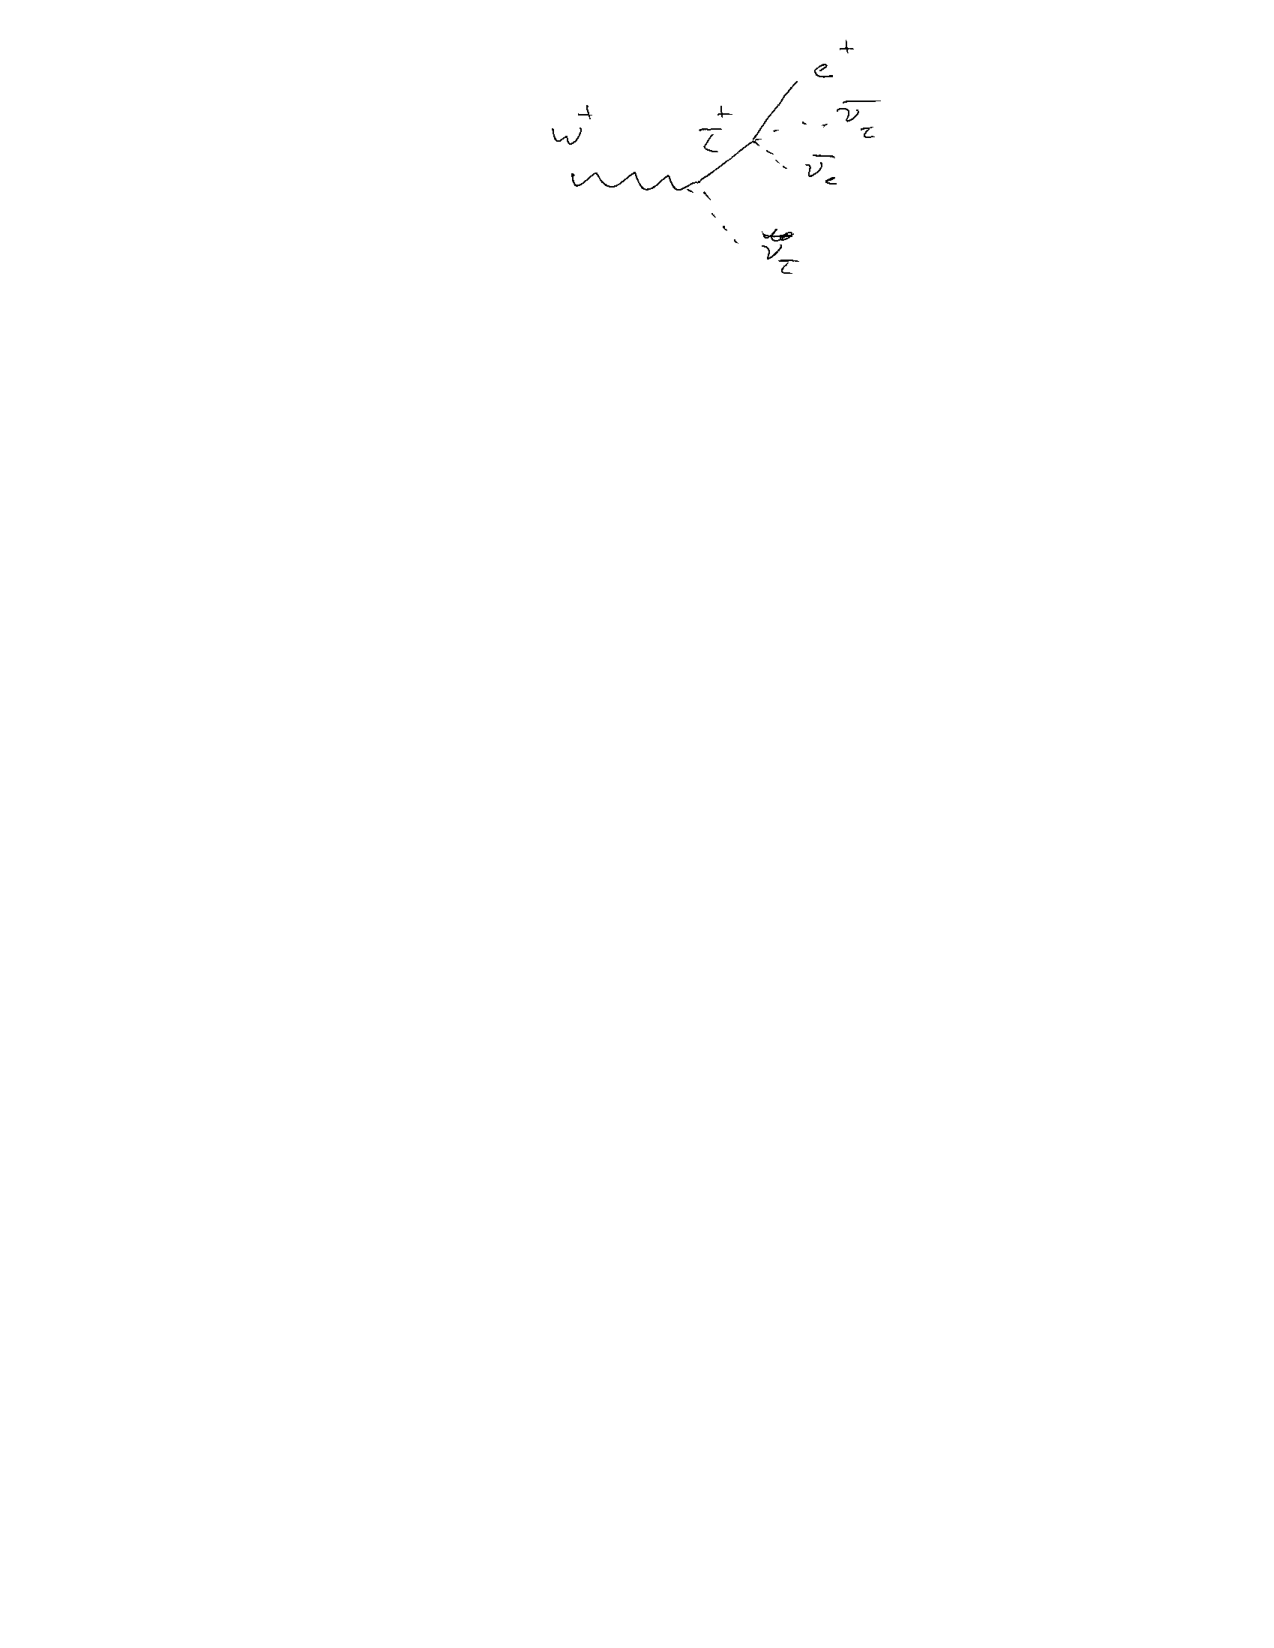
\includegraphics[width=0.3\textwidth]{./We3nu.pdf}
\ec
}
\item[b)]{ 
\be
Br(W\rightarrow \ell \nu)  = \frac{1}{\underbrace{3}_{\rmt{leptons}} + \underbrace{3}_{\rmt{color}} \times \underbrace{2}_{\rmt{2 quark generations}}} = \frac{1}{9} = 0.11
\ee
(Note the top-quark is heavier than the W, so the $W\rightarrow t, b $ decay is forbidden.)

Now,
\be
Br(\tau \rightarrow e \nu \bar{\nu})  = \frac{1}{\underbrace{2}_{\rmt{leptons}} + \underbrace{3}_{\rmt{color}} \times \underbrace{2}_{\rmt{1 quark generations}}} = \frac{1}{5} = 0.2
\ee
Here the $\tau$ can decay to two lepton generation (es and $\mu$ s), but only has enough mass to decay to one quark generation (u, d). 


So, 
\be
Br(W\rightarrow e + X) = \underbrace{\frac{1}{9}}_{W\rightarrow e\nu} + \underbrace{\frac{1}{9}}_{W\rightarrow \tau\nu} \times \underbrace{\frac{1}{5}}_{\tau\rightarrow e\nu}  = \frac{1.2}{9} = 0.13
\ee

}
\end{itemize}           

\textbf{4)  $W$ boson decays to electrons. } \hfill \textit{(3 points)}\\

\be
Br(W\rightarrow \ell \nu) \sim \frac{1}{9} 
\ee

for e or $\mu$ can include the decays through $\tau$s as in problem 3 to get $\frac{1.2}{9}$

\be
Br(WW\rightarrow e\mu + X) = 2 \times \left(\frac{1.2}{9}\right)^2 \sim 0.036
\ee
Factor of two becuase you can get $e^+\mu^-$ or $e^-\mu^+$


\textbf{6) Galactic Collisions.} \hfill \textit{(10 points)}\\
\begin{itemize}
\item[a)] { 
$N_{star} \sim 10^{11}$\hspace*{0.5in}
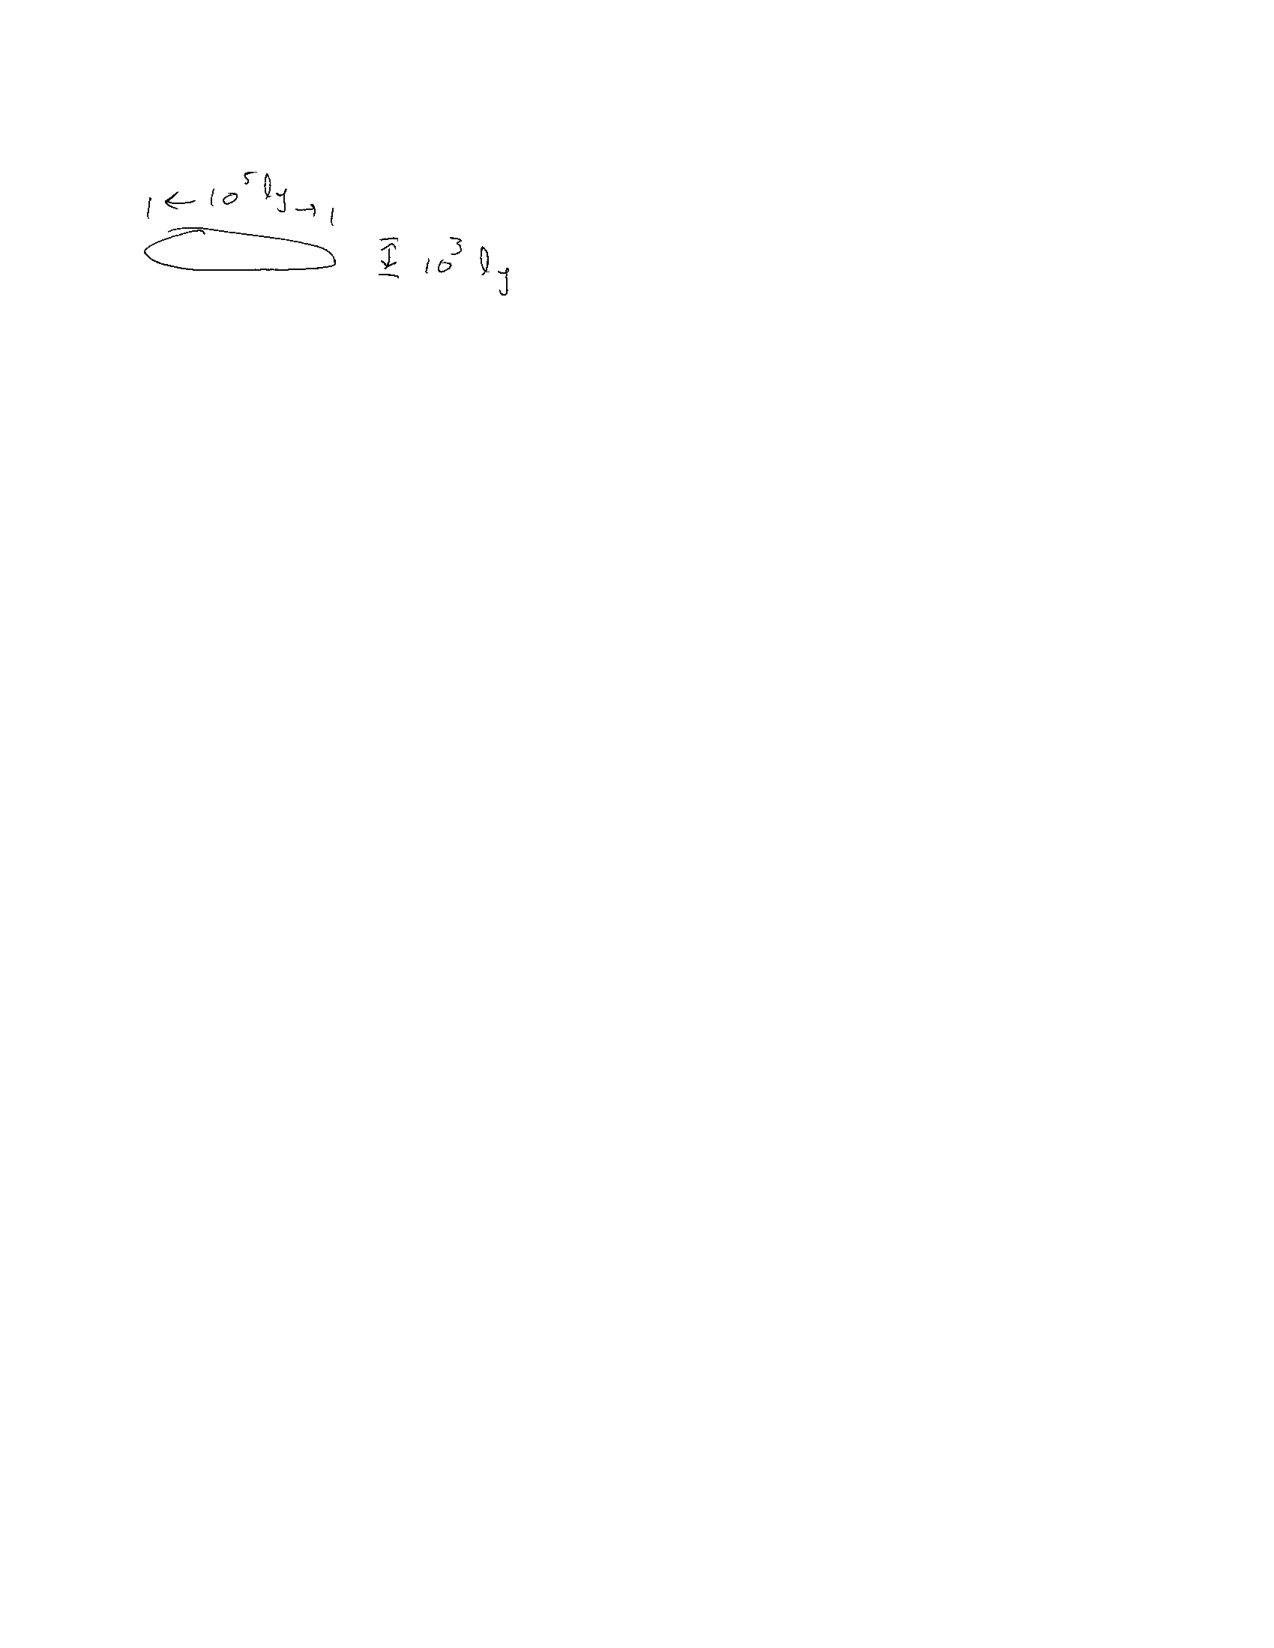
\includegraphics[width=0.3\textwidth]{./Galaxy.pdf}\hspace*{0.5in}
$v_{rel} \sim 10^5 m/s$

\be
\mathcal{L}_{galaxy} = \frac{N_A N_B |v_A - v_B|}{volume} \sim \frac{10^{22}\ 10^5\ m/s}{volume}
\ee

\be
volume = \pi (10^5/2\ ly)^2 \times 10^3\ ly = \frac{\pi}{4} 10^{13} (ly)^3 \sim 10^{13}(3.8\ m/s\ \pi 10^7 s)^3 = 10^{61}\ m^3
\ee

So,
\be
\mathcal{L}_{galaxy}  \sim \frac{10^{27}\ m/s}{10^{61}\ m^3} \sim 10^{-34} \frac{1}{m^2}\frac{1}{s} = 10^{-38} \frac{1}{cm^2}\frac{1}{s} 
\ee

\be
\mathcal{L}_{LHC}  \sim 10^{34} \frac{1}{cm^2}\frac{1}{s} 
\ee
So $\sim$ 72 orders of magnitude smaller !


}
\item[b)] {
In a galaxy,
\be
\frac{volume}{star} \sim \frac{10^{61}\ m^3}{10^{11}} \sim 10^{50}\ m^3
\ee


\be
\frac{distance}{star} \sim \left(\frac{volume}{star}\right)^{\frac{1}{3}} \sim 10^{50/3}\ m
\ee

So, 
\be
\frac{\rmt{<distance to star>}}{<R_*>} \sim \frac{10^{50/3}\ m}{7\cdot10^8\ m} \sim 10^8
\ee

In a proton bunch (with focusing magnets)  at the LHC, 
\be
\frac{volume}{proton} \sim \frac{10^{-10}\ m^3}{10^{11}} \sim 10^{-21}\ m^3
\ee

So
\be
\frac{distance}{proton} \sim \left(\frac{volume}{proton}\right)^{\frac{1}{3}} \sim 10^{-7}\ m
\ee

\be
\frac{\rmt{<distance to proton>}}{<R_p>} \sim \frac{10^{-21}\ m}{10^{-15}} \sim 10^8
\ee
Which is quite close !
}
\item[c)] {
For the galaxy,

\be
N_\rmt{collisions} = \int dt \mathcal{L} \times \sigma
\ee

Now, 
\be
\int dt = 10^9\ y \times (\pi 10^7)\ y/s
\ee
\be
\mathcal{L} = 10^{-34}\ m^{-2}s^{-1}
\ee
\be
\sigma = \pi (7\cdot 10^8\ m)^2
\ee
$\Rightarrow$ N-collisions $\sim 1$.

The LHC has baout $\sim 10$ proton collisions per bunch crossing. 

(Not so different!)

}
\end{itemize}

}
\end{document}
